%%
%% The first command in your LaTeX source must be the \documentclass command.
\documentclass[acmsmall,screen,10pt,nonacm]{acmart}
% \renewcommand\footnotetextcopyrightpermission[1]{}
% \settopmatter{printacmref=false}

%% \BibTeX command to typeset BibTeX logo in the docs
\AtBeginDocument{%
  \providecommand\BibTeX{{%
    \normalfont B\kern-0.5em{\scshape i\kern-0.25em b}\kern-0.8em\TeX}}}

% \usepackage[shortcuts]{extdash}
% \usepackage{multirow}
% \usepackage{graphicx}
\usepackage{xcolor}
\usepackage{soul}
\usepackage{listings}
\usepackage{courier}

\let\defaulttexttt\texttt
\renewcommand{\texttt}[1]{\defaulttexttt{\small{#1}}}

\lstset{basicstyle=\footnotesize\ttfamily,breaklines=true,captionpos=b}
\lstset{framextopmargin=50pt,frame=bottomline}

%% Rights management information.  This information is sent to you
%% when you complete the rights form.  These commands have SAMPLE
%% values in them; it is your responsibility as an author to replace
%% the commands and values with those provided to you when you
%% complete the rights form.
% \setcopyright{acmcopyright}
% \copyrightyear{2018}
% \acmYear{2018}
% \acmDOI{10.1145/1122445.1122456}

%% These commands are for a PROCEEDINGS abstract or paper.
\acmConference[Woodstock '18]{Woodstock '18: ACM Symposium on Neural
  Gaze Detection}{June 03--05, 2018}{Woodstock, NY}
\acmBooktitle{Woodstock '18: ACM Symposium on Neural Gaze Detection,
  June 03--05, 2018, Woodstock, NY}
\acmPrice{15.00}
\acmISBN{978-1-4503-XXXX-X/18/06}


%%
%% Submission ID.
%% Use this when submitting an article to a sponsored event. You'll
%% receive a unique submission ID from the organizers
%% of the event, and this ID should be used as the parameter to this command.
%%\acmSubmissionID{123-A56-BU3}

%%
%% The majority of ACM publications use numbered citations and
%% references.  The command \citestyle{authoryear} switches to the
%% "author year" style.
%%
%% If you are preparing content for an event
%% sponsored by ACM SIGGRAPH, you must use the "author year" style of
%% citations and references.
%% Uncommenting
%% the next command will enable that style.
%%\citestyle{acmauthoryear}

%%
%% end of the preamble, start of the body of the document source.
\begin{document}

\definecolor{UoC}{RGB}{137 33 27}
\begin{center}

\includegraphics[scale=0.2]{figures/UoC_logo.png}\\
\textcolor{UoC}{\textbf{UNIVERSITY OF CRETE}}\\
\textcolor{UoC}{\textbf{Computer Science Department}}
\vspace{3em}
\end{center}

%%
%% The "title" command has an optional parameter,
%% allowing the author to define a "short title" to be used in page headers.
\title{Single Sign-on for Internet Services}
\subtitle{Thesis submitted in partial fulfilment of the requirements for the degree of Computer Science}

\thanks{\small{This thesis was supervised by Prof. Angelos Bilas, co-supervised by Associate Prof. Polyvios Pratikakis and Antony Chazapis, PhD, Institute of Computer Science, FORTH, and submitted in December 2021}}

%%
%% The "author" command and its associated commands are used to define
%% the authors and their affiliations.
%% Of note is the shared affiliation of the first two authors, and the
%% "authornote" and "authornotemark" commands
%% used to denote shared contribution to the research.
\author{Loukas Merkouris}

\affiliation{%
  \department{Computer Science Department}
  \institution{University of Crete}
  \city{Heraklion}
  \country{Greece}
}
\email{csd3131@csd.uoc.gr}
%%
%% By default, the full list of authors will be used in the page
%% headers. Often, this list is too long, and will overlap
%% other information printed in the page headers. This command allows
%% the author to define a more concise list
%% of authors' names for this purpose.
\renewcommand{\shortauthors}{L. Merkouris}

%%
%% The abstract is a short summary of the work to be presented in the
%% article.
\begin{abstract}
% \section{Abstract}

The Internet hosts various amount of web applications, services and even more users.
These users, while using an application, often want to access their data that resides in another, third-party application, i.e., when a user uses an email application and wants to access his contacts that exist in another application, how will the email application eventually get his contacts?
In the old-fashioned way, the user had to hand over the credentials of his third-party application account to the application he eventually wants to get his data.
% but the user gave access to all of his data in the 3rd party application, including his password.
This was insecure for the user, the user gave access to all of his data in the 3rd party application, including his password.
With that method, the application that took his credentials could store them in plain text, the database could be hacked, and to revoke access, there was only one option; to change his password. With Single Sign-on (SSO), this problem no longer exists, as users can authorize the application to access a specific set of data residing elsewhere without disclosing passwords.
% , and give them access to a specific set of data.
Today there are many protocols and frameworks to achieve SSO, for users to be able to authorize and authenticate using third-party applications.
In this thesis, we examine SSO between Internet services using the OAuth 2.0 \cite{OAUTH} and OpenID Connect\cite{OIDC}  protocols, by implementing example web-based applications in Python using the Django\cite{Django} framework. We also extend one of the example applications to use a remote LDAP\cite{LDAP} server as a user directory instead of a local user database.

\end{abstract}


\maketitle

\section{Introduction}

Single Sign-on (SSO), is an authentication and authorization scheme where users can securely authorize, authenticate and gain access to multiple applications and websites by only logging in with a single username and password. In this project we use the OAuth 2.0 (OAuth) and OpenID Connect (OIDC) technologies to enable SSO. With SSO we can authorize and authenticate applications and access resources in a secure and fast way. Users can be in a local or a remote database. To enable authentication with users in a remote database, we use authentication via the Lightweight Directory Access Protocol (LDAP), which is commonly deployed for accessing and maintaining data in a company/organization server.
% , can also be used for authentication.

\section{Design}

To test SSO with OAuth and OIDC, we implemented 3 applications with Django, which is a high-level Python web framework that encourages rapid development and clean, pragmatic design. Django follows the model–template–views (MTV) architectural pattern. Django's primary goal is to ease the creation of complex, database-driven websites. The framework emphasizes reusability and ``pluggability'' of components, less code, low coupling, rapid development, and the principle of don't repeat yourself. Python is used throughout, even for settings, files, and data models. Django also provides an optional administrative create, read, update and delete interface that is generated dynamically through introspection and configured via admin models.



\subsection{OAuth 2.0}

OAuth is an open-standard authorization protocol that provides applications the ability for ``secure designated access''. For example, you can tell Facebook that it’s ok for YouTube to access your profile or post updates to your timeline without having to give YouTube your Facebook password. This minimizes risk in a major way: in the event, YouTube suffers a breach, your Facebook password remains safe. Hence, OAuth solves the problem of sharing resources, users don't have to disclose passwords or create accounts to use a service. It's easy for end-users to use, and the access can be revoked anytime.

Glossary of the components are:
\begin{itemize}
	
	\item \textbf{Resource Owner:} The user or system that owns the protected resources and can grant access to them.
	
	\item \textbf{Access Token:} A piece of data that represents the authorization to access resources on behalf of the Resource Owner.
	
	\item \textbf{Client:} A system that requires access to the protected resources. To access resources, the Client must hold the appropriate Access Token.
	
	\item \textbf{Authorization Server:} This server receives requests from the Client for Access Tokens and issues them upon successful authentication and consent by the Resource Owner. The authorization server exposes two endpoints: the Authorization endpoint, which handles the interactive authentication and consent of the user, and the Token endpoint, which is involved in a machine to machine interaction.
	
	\item \textbf{Resource Server:} A server that protects the user’s resources and receives access requests from the Client. It accepts and validates an Access Token from the Client and returns the appropriate resources to it.
	
	\item \textbf{Scopes:} A mechanism to limit an application's access to a user's account.
	
\end{itemize}

Scopes are used to specify exactly the reason for which access to resources may be granted. An application can request one or more scopes. This information is presented to the user in the consent screen, and the Access Token issued to the application will be limited to the scopes granted. Access Token is something like a key, while scopes specify which doors the key can open. Acceptable scope values and which resources they relate to are dependent on the Resource Server.

To enable the OAuth protocol in our project we created the \textbf{Provider}, acting both as the Resource Server and the Authorization Server, (the Resource and Authorization Servers can be separate applications, for this project they are the same), and the \textbf{Client}.
For implementing the Provider we used the \textbf{Django OAuth Toolkit}\cite{oauthtoolkit} package, which provides all the endpoints, data, and logic needed to add OAuth capabilities to our Django project.
With the toolkit, we made our Authorization Server issue Access Tokens to Client applications for a certain API.

Before our Application (the Client), can use the Authorization Server for authorization or authentication, we must first register the app. Once registered, the Client will be granted access to the API, subject to approval by its users. The registration process will automatically generate a unique Client\_id and Client\_secret, which are used so the Client and the Authorization Server establish a working relationship. The Authorization Server generates the Client ID and Client Secret (sometimes called the App ID and App Secret) and gives them to the Client to use for all future OAuth exchanges. The Client Secret must be kept secret so that only the Client and Authorization Server know what it is. This is how the Authorization Server can verify the Client. We have to provide the rest of the information:

\begin{itemize}

	\item \textbf{User:} The owner of the Application (e.g., a developer, or the currently logged in user).

	\item \textbf{Redirect URIs:} Applications must register at least one redirection endpoint before using the authorization endpoint. The Authorization Server will deliver the Access Token to the Client only if the Client specifies one of the verified redirection URIs.

	\item \textbf{Client type:} This value affects the security level at which some communications between the Client application and the Authorization Server are performed. For this project we use Confidential.

	\item \textbf{Authorization grant type:} Authorization Code.

	\item \textbf{Name:} This is the name of the Client application on the server, and will be displayed on the authorization request page, where users can allow/deny access to their data.

\end{itemize}

Authorization grant type refers to the way an application (the Client) gets an Access Token. OAuth defines several grant types and extensions can also define new grant types. Each grant type is optimized for a particular use case, whether that’s a web app, a native app, a device without the ability to launch a web browser, or server-to-server applications. We used the \textbf{Authorization Code} grant type, because when authorizing an application to access OAuth protected data with this grant type, the flow is always initiated by the user and the application can prompt users to click a special link to start the process. 
When a user clicks the link, the Client redirects the browser to the Authorization Server. If the user is not logged in, he will be prompted for a username and password. This is because the authorization page is login-protected by Django-OAuth-Toolkit. After login the user should see be presented with a form, including the scopes, to give his authorization to the Client application. User will flag the checkbox, click Authorize, and will be redirected again to the Client.

At this point the Authorization Server redirects the user to a special page on the Client passing in an Authorization Code and a special token that the Client will use to obtain the final Access Token. This operation is usually done automatically by the Client application during the request/response cycle. Access Tokens have a specific lifetime, given by the Authorization Server. Access Token has a Refresh Token as well which is used for a brand new Access Token when necessary, without repeating the authorization process, as it has no expire time.

\begin{figure}[htb]
	\centering
	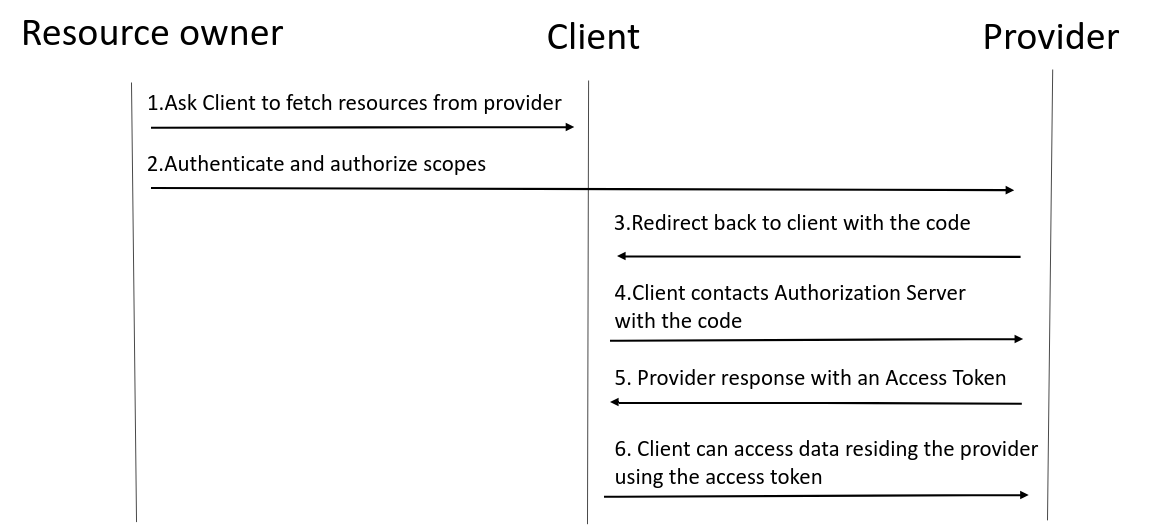
\includegraphics[scale=0.3]{figures/oauth.png}
	\caption{OAuth flow}
\end{figure}


	The OAuth flow (fig. 1):
	\begin{enumerate}
		\item The \textbf{Resource Owner}, want to allow the \textbf{Client}, to access data residing the \textbf{Provider}.
		
		\item \textbf{Resource Owner} clicks a special link to start the flow and the \textbf{Client} redirects browser to the \textbf{Authorization Server} and includes with the request the \textbf{Client ID}, \textbf{Redirect URI}, \textbf{Response Type}, and one or more \textbf{scopes} it needs. The \textbf{Authorization Server} verifies the user, and if necessary prompts for a login, then presents user with a consent form based on the scopes requested by the \textbf{Client}. \textbf{Resource Owner} grant (or deny) permission.
		
		\item The \textbf{Authorization Server} redirects back to \textbf{Client} using the \textbf{Redirect URI} along with an \textbf{Authorization Code}.
		
		\item The \textbf{Client} contacts the \textbf{Authorization Server} directly (does not use the Resource Owner’s browser) and securely sends its \textbf{Client ID}, \textbf{Client Secret}, and the \textbf{Authorization Code}.
		
		\item The \textbf{Authorization Server} verifies the data and responds with an \textbf{Access Token}.
		
	\end{enumerate}
The Client can now use the Access Token to send requests to the Resource Server for accessing data. OAuth is used for generic authorization; for authentication, we need to create an API endpoint at the Provider and call it to learn the user's information.


%\hl{Add a note that OAuth is used for generic authorization. For authentication, we then need to create an API endpoint at the server and call it to learn the user's ID, username, etc.}

\subsection{OpenID Connect}

OAuth is designed only for authorization, for granting access to data and features from one application to another. After the OAuth flow, usually the first step for the Client is to get information about the Resource Owner (the end-user), by sending the proper request to the Resource Server. That step can be avoided by using OIDC.
OpenID Connect (OIDC) is a thin layer that sits on top of OAuth that adds login and profile information about the person who is logged in. Establishing a login session is often referred to as authentication, and information about the person logged in (i.e. the Resource Owner) is called identity. When an Authorization Server supports OIDC, it is sometimes called an identity provider, since it provides information about the Resource Owner back to the Client. OIDC flow looks the same as OAuth, the only differences are that in the initial request, a specific scope of \textbf{openid} is used, and the Server responds with an Access Token and A JSON Web Token (JWT) that contains the information about the Resource owner.

\begin{figure}[htb]
	\centering
	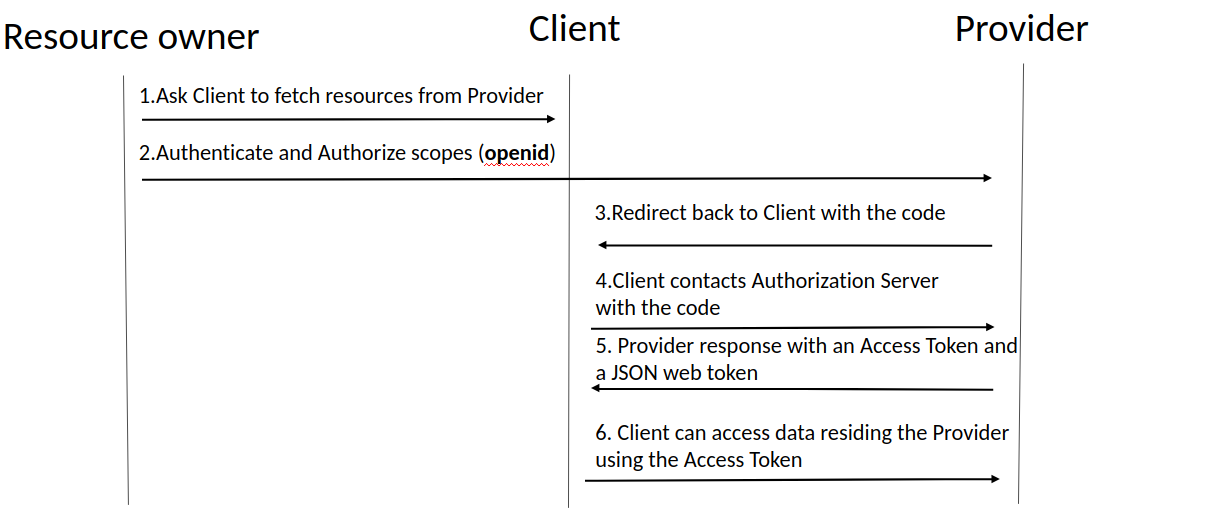
\includegraphics[scale=0.4]{figures/OIDC.png}
	\caption{OIDC flow}
\end{figure}

OIDC flow (fig. 2) is the same with the OAuth flow with two extra steps:

\begin{itemize}
	
	\item In step 2, the \textbf{Authorization Server} presents user with a consent form based on the scopes and a specific scope \textbf{openid} is used requested by the \textbf{Client}.
	
	\item In step 5, the \textbf{Authorization Server} verifies the data and responds with an \textbf{Access Token} and a \textbf{JSON Web Token}.
\end{itemize}	

Finally, the Client use the Access Token to access data  that resides to the Resource Server on behalf of the Resource Owner; using the JWT the Client has information about the Resource Owner.
	

\subsection{Lightweight Directory Access Protocol}

The Lightweight Directory Access Protocol (LDAP) is one of the core authentication protocols that was developed for directory services. LDAP historically has been used as a database of information, primarily storing information like \textbf{users}, \textbf{attributes about those users}, \textbf{group membership privileges} and more. This information was then used to enable authentication to IT resources such as an application or server. They would be pointed to the LDAP database, which would then validate whether that user would have access to it or not. That validation would be done by passing a user’s credentials. LDAP authentication follows the client/server model. In this scenario, the client is generally an LDAP-ready system or application that is requesting information from an associated LDAP database and the server is, of course, the LDAP server. The server side of LDAP is a database that has a flexible schema. In other words, not only can LDAP store username and password information, but it can also store a variety of attributes including address, telephone number, group associations, and more. As a result, a common LDAP use case is to store core user identities. In doing so, IT can point LDAP-enabled systems and applications (for example) to an associated LDAP directory database, which acts as the source of truth for authenticating user access.

We add LDAP authentication in our OIDC Provider using the \textbf{auth-ldap} \cite{ldapauth} package. This package is a Django authentication backend that authenticates against an LDAP service (in our case FORTH'S LDAP Server). Configuration can be as simple as a single \textbf{distinguished name} (DN) template, but there are many rich configuration options for working with users, groups, and permissions. For authentication with the LDAP server, we need to add the LDAP backend from the auth-ldap package and point to the LDAP server.

Now that we can talk to the LDAP server, the next step is to authenticate a username and password. There are two ways to do this, called \textbf{search/bind} and \textbf{direct bind}. The first one involves connecting to the LDAP server either anonymously or with a fixed account, and searching for the distinguished name of the authenticating user. Then we can attempt to bind again with the user’s password. The second method is to derive the user’s DN from his username and attempt to bind as the user directly.

We used Direct Bind, to skip the search phase. All we need to do was to set \verb|AUTH_LDAP_USER| \verb|_DN_TEMPLATE| to a template that will produce the authenticating user’s DN directly. This template should have one placeholder, \%(user)s. By setting \verb|AUTH_LDAP_USER_ATTR_MAP| we are able to match our user's model attributes with the LDAP user.
With these settings, we are able to connect to an LDAP server. When the LDAP server authenticates the user's credentials, the auth-ldap backend will return an LDAP\_user and will create a Django user on return with the attributes that were given.

\begin{figure}[htb]
	\centering
	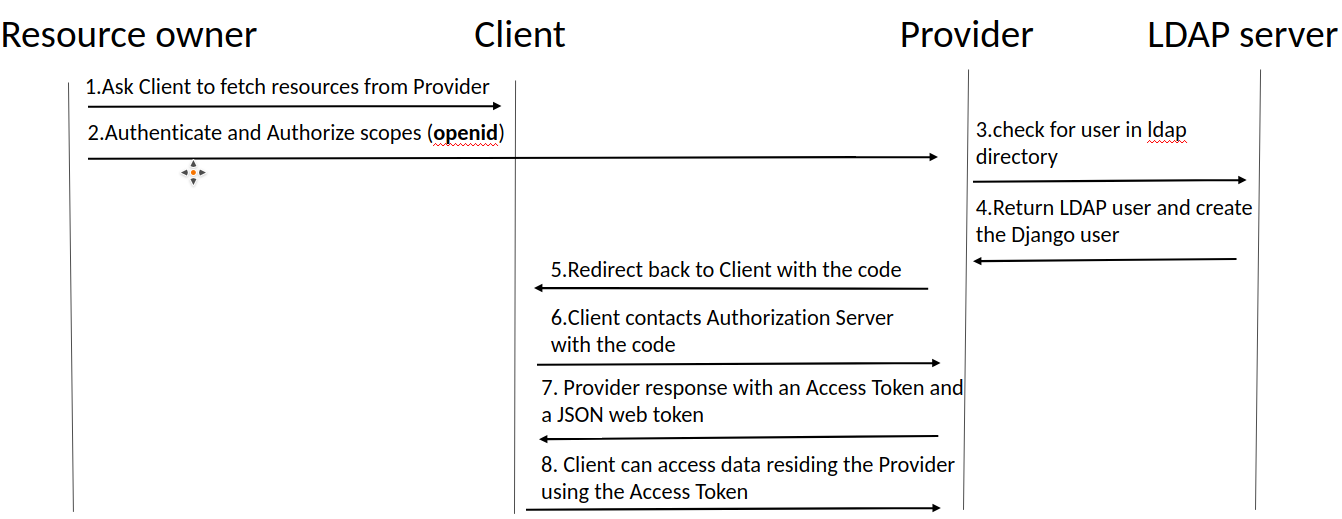
\includegraphics[scale=0.3]{figures/LDAP.png}\\
	\caption{OIDC with LDAP flow}
\end{figure}

The authentication scheme from a LDAP database with OIDC flow (fig. 3), its the same with OIDC flow, the only difference is that the Provider search for users in a remote database:

\begin{itemize}

	
	\item In step 3, the \textbf{Authorization Server }validates given credentials with the remote LDAP database. 
	
	\item In step 4, if the user exists, returns the user and create a local Django user. The \textbf{Authorization Server} presents user with a consent form based on the scopes (like OIDC, a specific scope \textbf{openid} is used) requested by the \textbf{Client}. User grant (or deny) permission.
	
	
\end{itemize}

The Resource Owner, is authenticated to the Client using his credentials that exists in a remote database and Client has all the profile information of the LDAP user.


\section{Implementation}

In this section, we will take a closer look at how the implementation works (fig. 6). Starting from the Client and following the Providers, showing how we add the components on each application, what extra code we use to enable different authentication and authorization schemes. 


\subsection{The Client}

The client is a Django application with a custom user model. Django comes with a user authentication system. It handles user accounts, groups, and permissions, using cookie-based user sessions. For authenticating, Django searches for the given user's credentials in its backends, and if the user exists, Django authenticates and redirects the user to the proper URL. We implement 2 custom backends for the Client application, one for searching users in the OAuth Provider (fig. 4) and one for OIDC Provider (fig. 5).

We installed the Python \textbf{django-social-auth} \cite{djangosocial}, which is a package for authenticating against third-party applications, like GitHub, Google, Facebook, and other websites. It also contains the base class for the OAuth authentication backend, called BaseOAuth2. In our custom OAuth backend, we override some of the BaseOAuth2 components, so the backend knows where to search for the Authorization Server, where to get the token, and other details.

For the OIDC custom backend, all we need to do is to overwrite the OpenIdConnectAuth class, which django-social-auth also provides, provide the name of our backend and the URL of the Authorization Server. The Client is ready to redirect the Resource User to the Providers and initiate the OAuth/OIDC process.


\begin{figure}[htb]
	\centering
	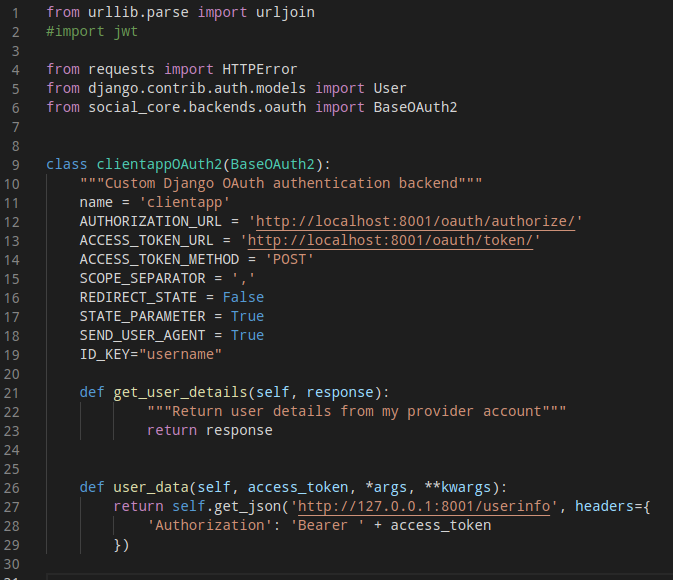
\includegraphics[scale=0.5]{figures/clientapp.png}
	\caption{OAuth custom backend}
\end{figure}


\begin{figure}[htb]
	\centering
	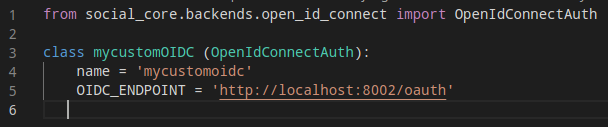
\includegraphics[scale=0.6]{figures/customOIDC.png}
	\caption{OIDC custom backend}
\end{figure}


\subsection{The Providers}

As mentioned, we used the Django-OAuth-Toolkit for the implementation of the Providers. To enable the Django-OAuth-Toolkit we need to add \verb|"oauth2_provider"| in installed apps and add the middleware \verb|"oauth2_provider.middleware.OAuth2TokenMiddleware"| in settings.py. The next step is to add the toolkit's backend for OAuth requests by adding \verb|"oauth2_provider.backends.OAuth2Backend"| in authentication backends, and specify the scopes as: \\ \verb|'SCOPES': {'read': 'Read scope', 'write': 'Write scope'}|.
In urls.py we add an extra URL: \verb|path('userinfo', user_info_secret)|, which is the endpoint in order for the custom backends know where to search for the user's information after authenticating. We also provide the OAuth Toolkit's endpoints by adding \verb|url(r"^oauth/", include| \verb|('oauth2_provider.urls', namespace='oauth2_provider'))|.


For the OIDC Provider implementation, we need to do two more steps. Add the specific scope of \textbf{openid} in \verb|'SCOPES'|, and create a \verb|CustomOAuth2Validator| method, which is used for mapping the user's info from the OIDC Provider to the Client. 



Finally, we have to register the Client in both of the Providers and set the correct Client\_id and Client\_secret in Client's settings.py. For the OIDC implementation, we need to provide an algorithm, which is used for signing the JWT that the Provider sends back to Client, for which we used the RS256 algorithm. After the registration process, Providers are ready to give Access Tokens to Client.

In the OIDC implementation, we also add the LDAP authentication scheme, by setting:

\begin{itemize}

	\item \verb|AUTH_LDAP_SERVER_URL|: Points to the LDAP server.

	\item \verb|AUTH_LDAP_BIND_DN|: Username.

	\item \verb|AUTH_LDAP_BIND_PASSWORD|: Password.

	\item \verb|AUTH_LDAP_USER_DN_TEMPLATE|: How to find the user.

	\item \verb|AUTH_LDAP_USER_ATTR_MAP|: What attributes we want to populate the Django user who is gonna be created.

\end{itemize}

The hole implementation is shown in fig. 6. The Resource Owner wants to use the Client which is a Django application with two custom backends and can authenticate the user via OAuth or OIDC implementation of the Providers. The OAuth and OIDC Providers are Django apps and using the Django-oauth-toolkit


\begin{figure}[htb]
	\centering
	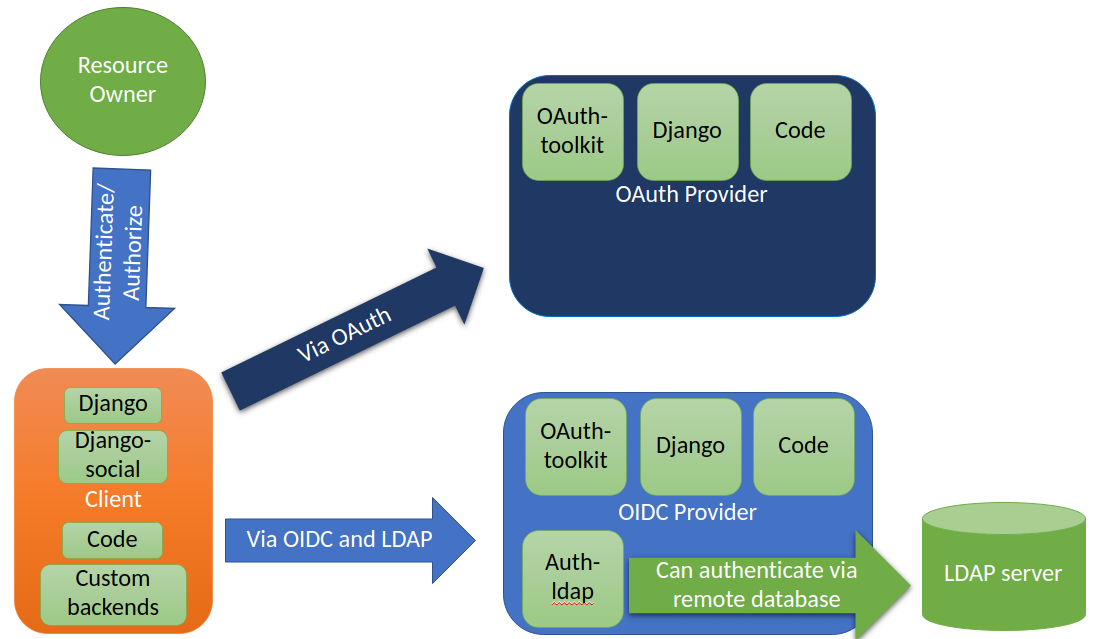
\includegraphics[scale=0.5]{figures/implementation.png}
	\caption{Implementation}
\end{figure}


\section{Conclusion}
We managed to enable both OAuth and OIDC protocols to authorize and authenticate between Django applications. We built two applications with Django, and made them Providers with Django-OAuth-Toolkit, acting as Resource Servers and Authentication Servers, one for OAuth and one for OIDC. With Django we create the Client, an application for users to login via the Providers, made possible by creating 2 custom backends (one for OAuth and one for OIDC) which override the base OAuth class that the django-social-auth provides and we managed to authenticate and authorize from the Client application. With the auth-ldap package, we added LDAP authentication functionality to the OIDC implementation of the provider using FORTH's LDAP server. Code is available at \href{https://github.com/CARV-ICS-FORTH/django-oauth2-oidc-example}{https://github.com/CARV-ICS-FORTH/django-oauth2-oidc-example.}


\begin{acks}
% I would like to thank Prof. Agelos Bilas for allowing me to implement my thesis in his lab, and Mr. Antonis Xazapis for providing guidance, giving valuable comments and suggestions during this work
I would like to thank all the membes of the CARV lab at Forth for their help and support, specialy Mr. Antony Chazapis for providing guidance, giving valuable comments and suggestions during this work.
%\hl{Probably just thank the members of the CARV lab at FORTH for their help, etc.}
\end{acks}



\bibliographystyle{plain} % We choose the "plain" reference style
\bibliography{acmart} % Entries are in the acmart.bib file
\end{document}
